\chapter{Opis tabel}
\label{chap:opistabel}

\begin{figure}[ht!]
\centering
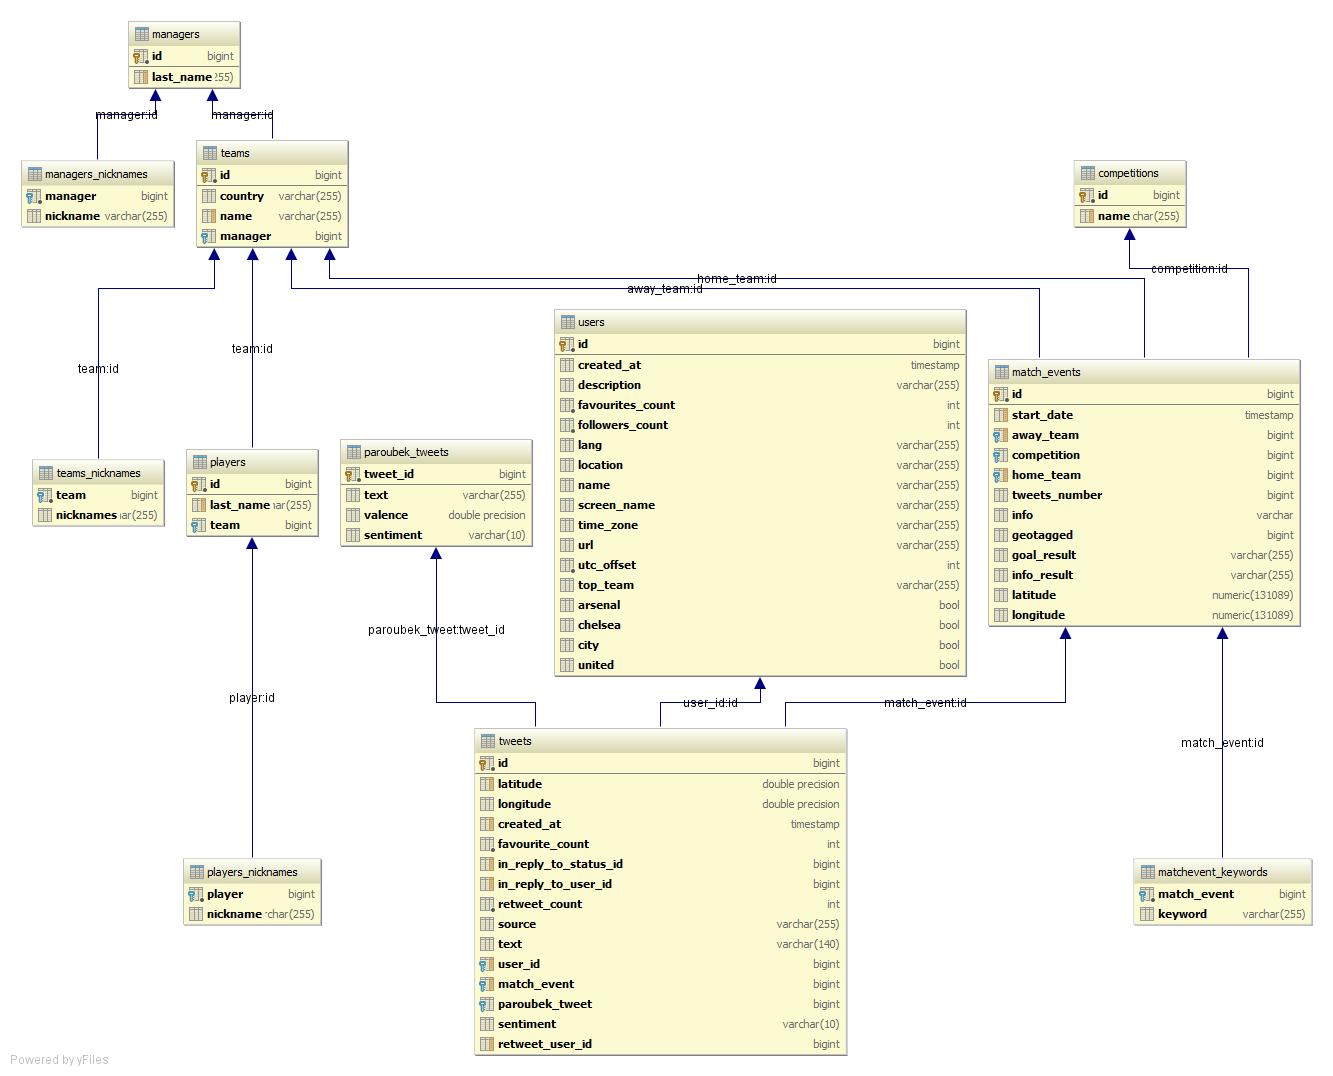
\includegraphics[width=160mm]{img/db-schema-intellij.png}
\caption{Schemat bazy danych}
\label{image:schemat-bazy-dodatek}
\end{figure}

\begin{description}
  \item[tweets] najważniejsza tabela w systemie. Tutaj gromadzone były
  nasłuchiwane tweety. Każdy tweet ma swój unikalny identyfikator \textit{id},
  informacje o dacie utworzenia \textit{created\_at}, autorze \textit{user\_id},
  współrzędnych geograficznych \textit{latitude} i \textit{longitude} oraz
  meczu, podczas którego tweet został wysłany \textit{match\_event}. Tabela ta
  powiązana jest z tabelami \textit{users}, \textit{match\_events} oraz
  \textit{paroubek\_tweets}.

  \item[paroubek\_tweets] tabela zawierająca przeliczone informacje o
  sentymencie tweetów. Każdy wiersz odwołuje się bezpośrednio kluczem obcym do
  tabeli \textit{tweets}. Kolumna \textit{text} zawiera oczyszczoną postać
  tweeta, \textit{sentiment} zawiera obliczoną klasę sentymentu (pozytywny,
  negatywny) a w \textit{valence} znajduje się wartość wyliczona przez algorytm
  użyty w analizie sentymentu.
 
  \item[users] tabela zawierająca informacje o użytkownikach będących autorami
  wpisów z Twittera. Rekordy były tworzone równocześnie z nasłuchiwaniem tweetów.
  W wyniku obliczeń i eksperymentów została wzbogacona o informacje o ulubionej
  drużynie kibica \textit{top\_team} oraz o byciu zwolennikiem lub przeciwnikiem
  poszczególnych klubów \textit{arsenal}, \textit{chelsea}, \textit{city},
  \textit{united}.
  
  \item[match\_events] tabela zawierająca informacje o nasłuchiwanych
  spotkaniach. Czas rozpoczęcia, uczestniczące drużyny, współrzędne stadionu.
  Powiązania jest z innymi tabelami (\textit{teams},
  \textit{matchevent\_keywords}), z których budowane były zbiory słów kluczowych
  do nasłuchiwania.
\end{description}